\documentclass[11pt]{article}
\usepackage[utf8]{inputenc}
\usepackage[french]{babel}
\usepackage{graphicx}
\usepackage[T1]{fontenc}
%\usepackage{amss}
\usepackage{amsmath}
\usepackage{amsfonts}
\usepackage{amssymb}

\newcommand\comment{}
\def\N{\mathbb N}
\def\R{\mathbb R}
\def\Q{\mathbb Q}
\def\Z{\mathbb Z}
\begin{document}
\title{PARTIEL I31, 2015}
\date{}\maketitle


\section{Problème 1}

1. Indiquez les dates au plus tôt et au plus tard sur ce graphe, 
et soulignez le chemin critique. 

\begin{center}
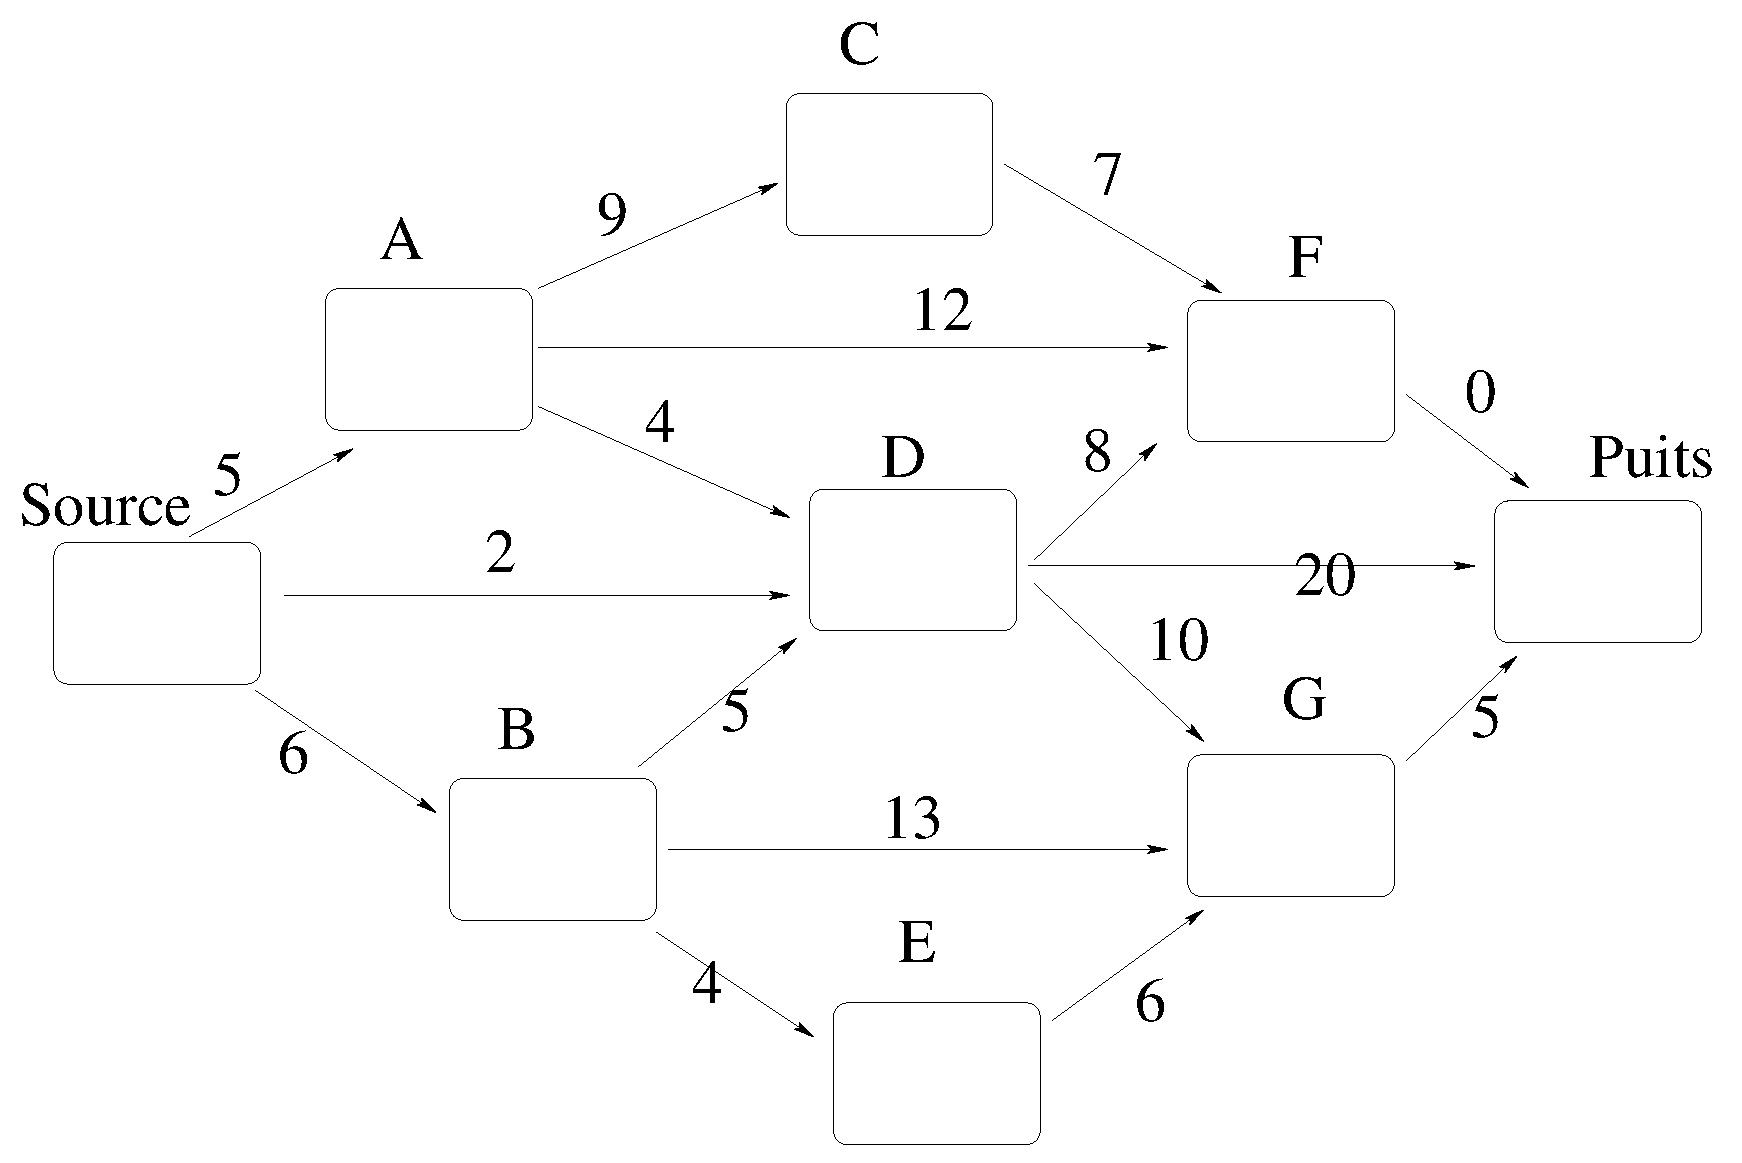
\includegraphics[width=0.7\linewidth]{critique.eps}
\end{center}

2. Que faire si le graphe a plusieurs sommets sources (ou puits) ?

3. Vous pouvez supposer que le graphe est acyclique, qu'il a un seul sommet source, un seul sommet puits, et que les durées sur les arcs sont non négatives.
Donnez la définition, en français, de la date au plus tôt. Prévoyez bien tous les cas.

4. Donnez la définition, en français, de la date au plus tard.

5. Quand un sommet est-il critique~?

\section{Euclide et Bézout}
1. Calculer PGCD(330, 210) avec l'algorithme d'Euclide.

2. Calculer $u\in \Z, v\in \Z$ minimaux (minimisant $u^2+v^2$) tels que $330u+210v=\mbox{PGCD}(330, 210)$. 

3. Donnez une formule avec un paramètre permettant de générer toutes les paires  $(u, v)$ telles
que $330u+210v=\mbox{PGCD}(330, 210)$.

\section{Quizz}

1. Citez deux problèmes indécidables en informatique.

2. Quand dit-on qu'un problème est difficile en informatique.

3. Citez deux problèmes solubles en informatique, mais difficiles.

4. Donnez deux algorithmes efficaces pour trier des nombres flottants, en utilisant des comparaisons. Dire quelle est la complexité de ces deux algorithmes.

5. Donnez le nom de trois algorithmes calculant les plus courts chemins dans un graphe.


\section{Dessinez le graphe d'un jeu de Nim}
Deux joueurs jouent à tour de rôle. Sur la table, il y a trois tas de pions~:
deux tas de 2 pions, et un tas de 1.
Albert commence, Bertrand joue en second. Chacun choisit un tas (non vide) et  un seul,
et en retire un nombre entier  non nul  de pions~; il peut retirer  tous les pions du tas s'il le souhaite~; le premier joueur qui ne peut plus retirer de pions
a perdu, ou, le premier joueur qui enlève tous les pions restant dans le dernier tas a gagné. 

1. Dessinez le graphe des coups possibles~; chaque état (tel (3, 2, 1) initialement) est représenté par un sommet~; un arc va d'un sommet $s$ à un sommet $t$ quand il est possible de passer en un coup de $s$ à $t$. 
Dessinez les sommets par niveaux~; le niveau $0 \le n \le 6 $ contient les états où la somme des nombres de pions vaut $n$. Par exemple le niveau 2 contient
les états $(1, 1), (2)$. N'utilisez qu'un seul sommet pour des états équivalents~: $(2, 1, 1)=(1, 2, 1)=(1, 1, 2)$, et éliminez les $0$ qui sont inutiles. Attention~: n'oubliez pas d'arc~!

2. Quel joueur, Albert ou Bertrand, est sûr de gagner, s'il joue intelligemment, bien sûr~? Vous entourerez les sommets G pour gagnant, ou P pour perdant~: un sommet est gagnant si le joueur qui y arrive peut toujours gagner, quels que soient les coups joués par l'adversaire. 

3. Décrivez l'algorithme que vous avez utilisé.


4. Dans un graphe orienté acyclique (c'est le cas ici), un noyau $N$ est 
un sous-ensemble de sommets du graphe tel que~: si $s$ est dans $N$, tous ses voisins sont hors de $N$~; si $s$ est hors de $N$, il existe au moins un arc vers un sommet $t$ qui se trouve dans $N$. Quel est le lien avec le problème précédent~? 

\newpage
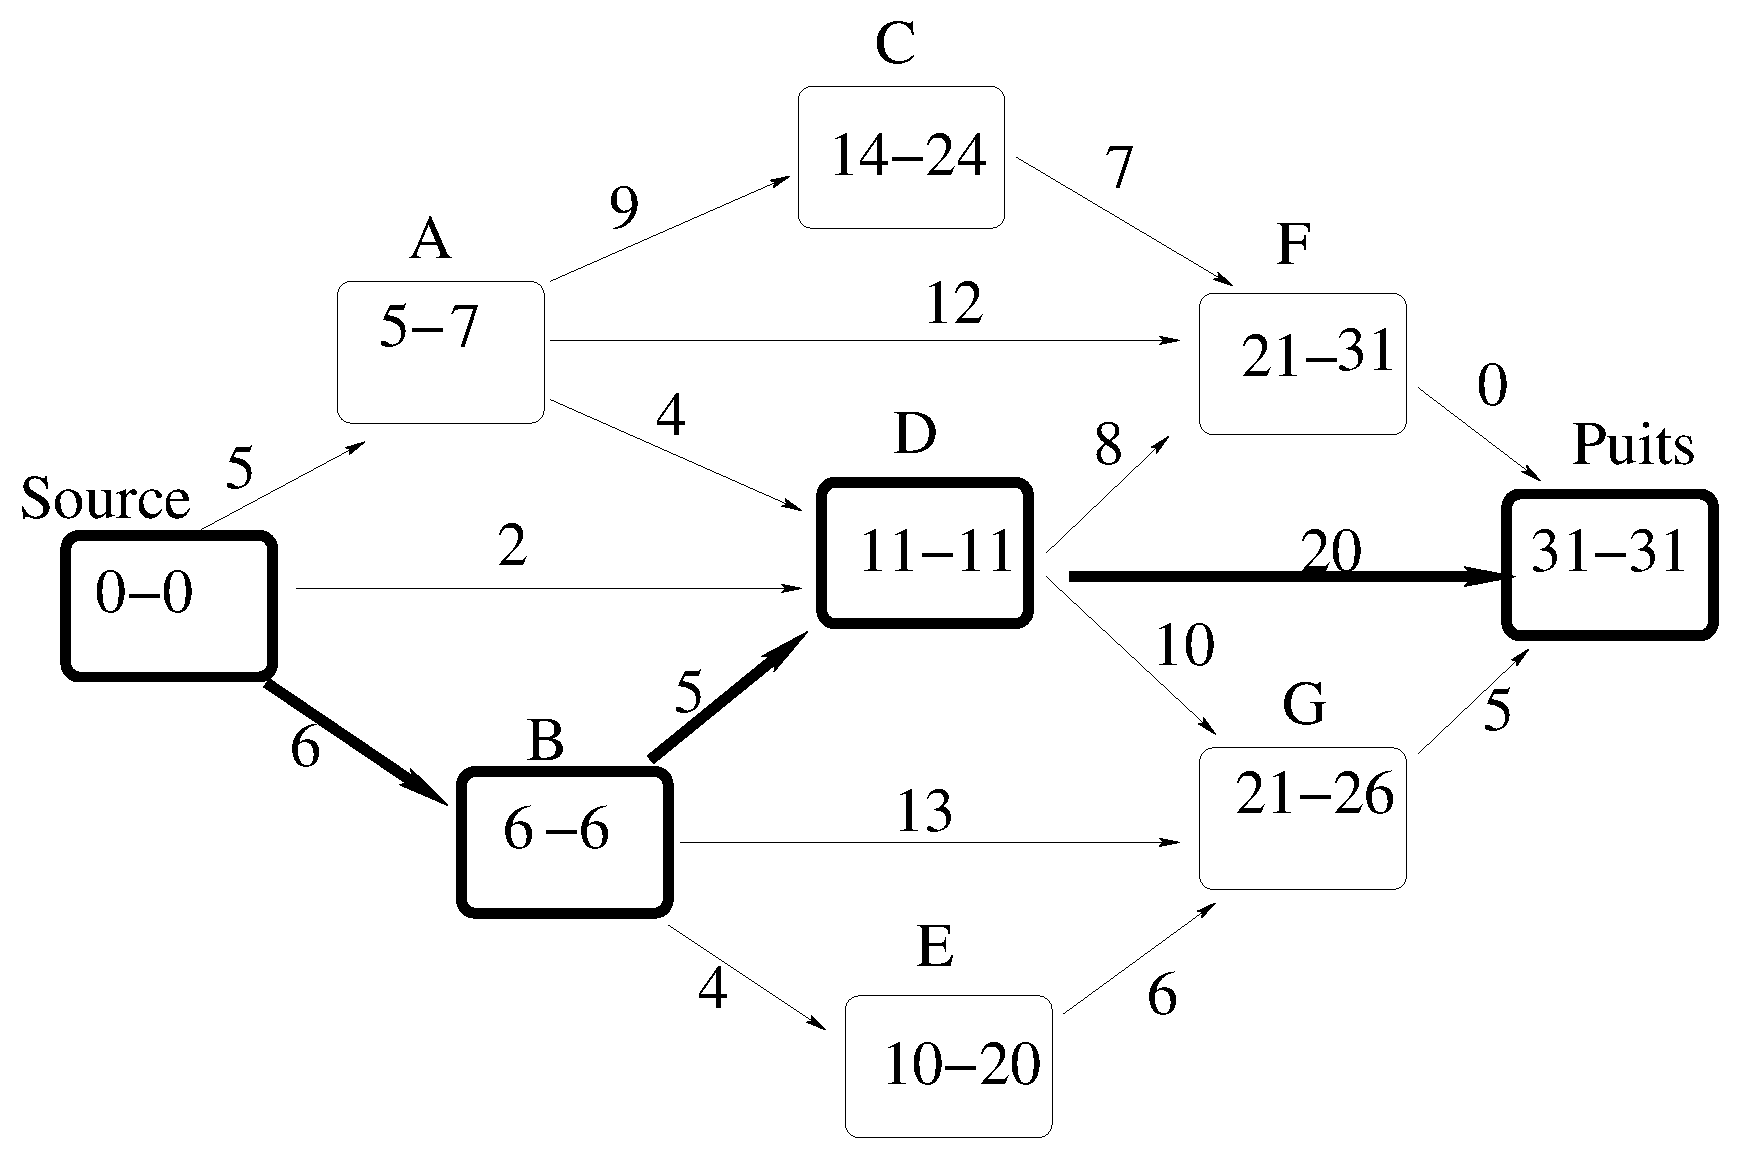
\includegraphics[width=0.95\linewidth]{critique_solution.eps}

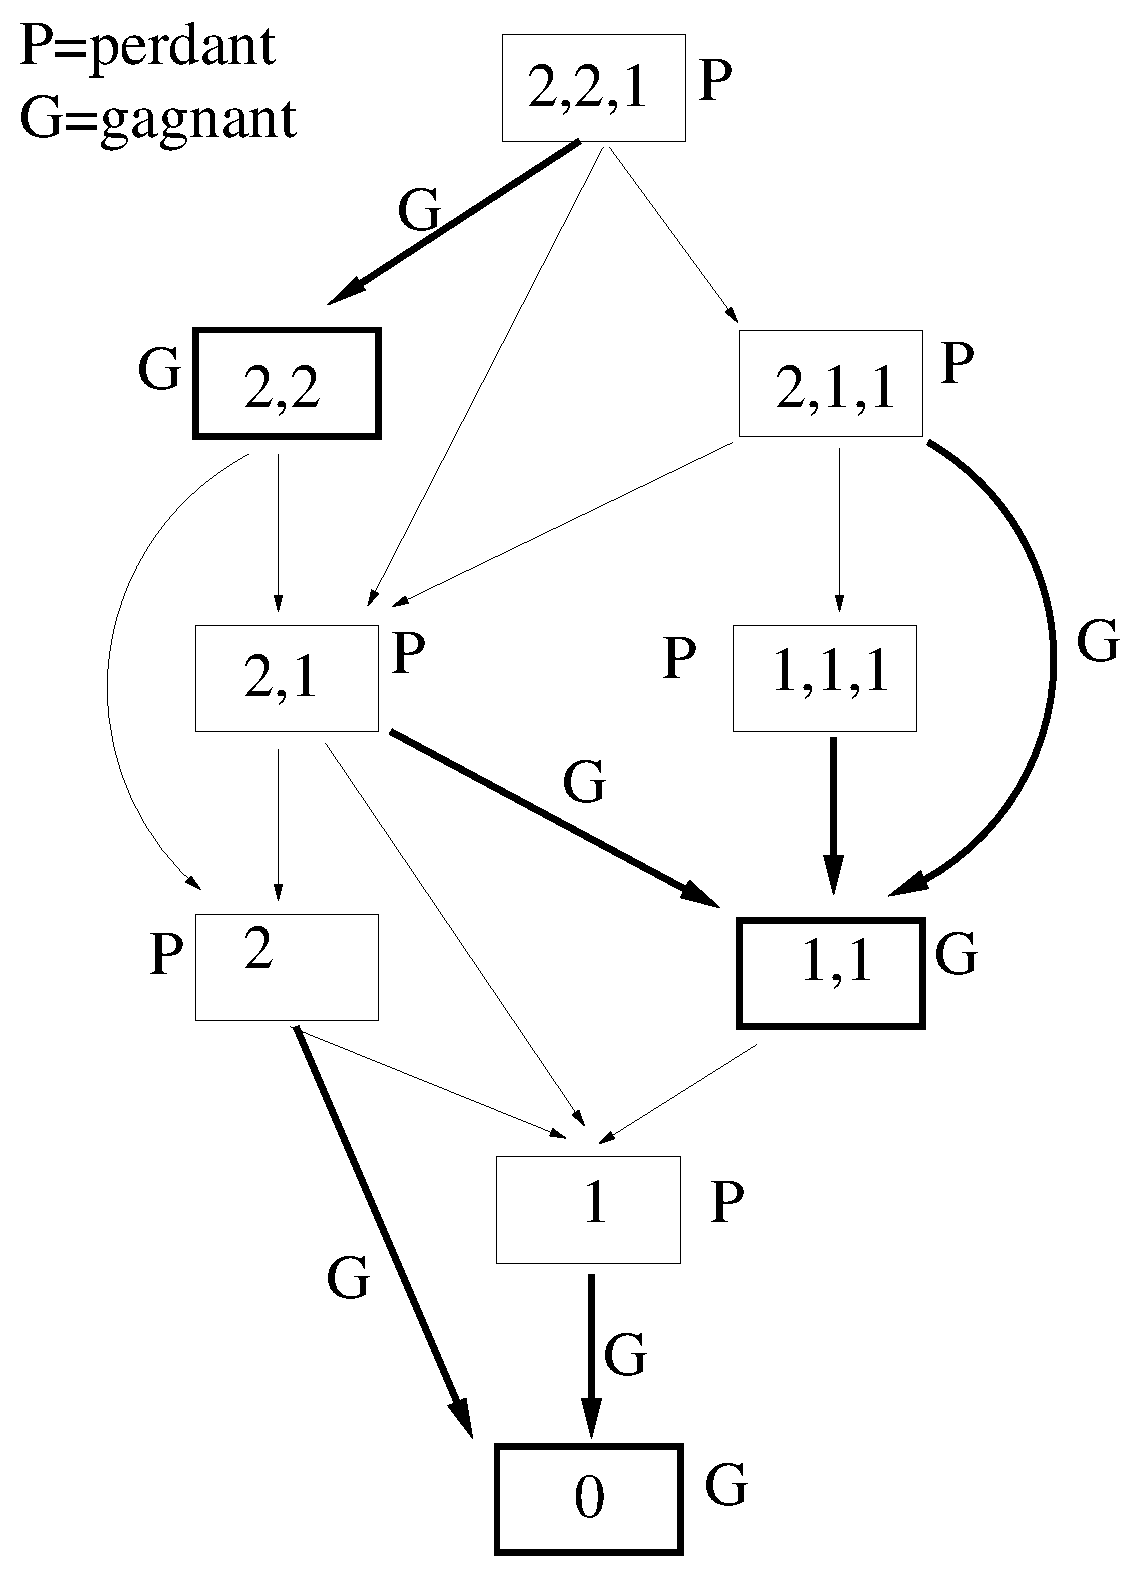
\includegraphics[width=0.6\linewidth]{nim.eps}

\end{document}
